%% uctest.tex 11/3/94
%% Copyright (C) 1988-2004 Daniel Gildea, BBF, Ethan Munson.
%
% This work may be distributed and/or modified under the
% conditions of the LaTeX Project Public License, either version 1.3
% of this license or (at your option) any later version.
% The latest version of this license is in
%   http://www.latex-project.org/lppl.txt
% and version 1.3 or later is part of all distributions of LaTeX
% version 2003/12/01 or later.
%
% This work has the LPPL maintenance status "maintained".
% 
% The Current Maintainer of this work is Daniel Gildea.
\documentclass[11pt]{ucthesis}
\setlength\parindent{0.5cm}

%% The graphicx package provides the includegraphics command.
\usepackage{graphicx}
\graphicspath{{../../../latex/graphics/}{./figures/}{./graphics/}}
%% The amssymb package provides various useful mathematical symbols
\usepackage{amssymb}
\usepackage{amsmath}
\usepackage{amsthm}
\usepackage{relsize} % \mathlarger
\usepackage{mathtools}
\usepackage{braket}
\usepackage{enumerate, enumitem}
\usepackage{caption}
\usepackage{subcaption}
\usepackage{float}

\def\dsp{\def\baselinestretch{2.0}\large\normalsize}
\dsp

\newcommand{\vect}[1]{{\it{\boldsymbol{#1}}}}

\begin{document}
% Declarations for Front Matter

\title{FASTPas - Fast Predictive Aerial Scanning}
\author{Sargis S Yonan}
\degreeyear{2018}
\degreemonth{June}
\degree{MASTER OF SCIENCE}
\chair{Professor Gabriel Hugh Elkaim}
\committeememberone{Professor Numero Dos}
\committeemembertwo{Professor Numero Tres}
\numberofmembers{3} %% (including chair) possible: 3, 4, 5, 6
\deanlineone{Dean Tyrus Miller}
\deanlinetwo{Vice Provost and Dean of Graduate Studies}
\deanlinethree{}
\field{COMPUTER ENGINEERING}
\emphasis{ROBOTICS AND CONTROL}
\campus{Santa Cruz}

\begin{frontmatter}

\maketitle
\copyrightpage

\tableofcontents
\listoffigures
\listoftables

\begin{abstract}
The use of the Kriging Method, a popular interpolation tool, offers a prediction and a variance of prediction, but is computationally expensive because of constant fitting procedures. We can exploit the Kriging variances generated by our prediction to motivate the UAVs to autonomously steer in the areas of least confidence until a minimum confidence in prediction is achieved for an entire unknown field. By designing a computational efficient algorithm based on a Universal Kriging Method, the system is feasible and could benefit a large group of potential users.
\end{abstract}

\begin{dedication}
\null\vfil
{\large
\begin{center}
yerba mate
\vspace{12pt}
\end{center}}
\vfil\null
\end{dedication}


\begin{acknowledgements}
yerba mate in a glass bottle, but can will do
%who helped me make sense of the various concepts involved in and out of this project. I would like to extend my thanks to the rest of the Autonomous Systems Lab at UC Santa Cruz for the support and motivation to continue this project everyday.
\end{acknowledgements}

\end{frontmatter}
\chapter{Introduction}
Unmanned Aerial Vehicles (UAVs) have become more prevalent in fields of work and study that benefit from having a birds eye view on a given situation. Firefighter teams have been using UAVs to find the origin of fires, and find the locations of fires. UAVs can be useful in the event of an oil spill, in order to find the impacted zones faster. Scientific researchers have been using aerial thermal imaging to determine rates of change in ice growth and melting, and thermal exchange between the ocean and atmosphere.
\par
The use of autonomous UAVs could benefit rescue teams, firefighters, scientific research, and private sector industries in the interest of time and data discovery. Using a single or multiple UAVs in a flying network, an area with fields of interest can be scanned efficiently completely autonomously. By simply drawing on a map the general area wished to be scanned by the autonomous fleet, a deployed pod of these UAVs can stream back, to a ground station, live aerial information. This mapping time can be greatly reduced with the use of statistical interpolation techniques that help the pod or single UAV avoid having to scan an entire region, but rather, have the UAVs scan the areas with the lowest level of confidence in prediction.
\par
The use of the Kriging Method, a popular interpolation tool, offers a prediction and a variance of prediction, but is computationally expensive because of constant fitting procedures. We can exploit the Kriging variances generated by our prediction to motivate the UAVs to autonomously steer in the areas of least confidence until a minimum confidence in prediction is achieved for an entire unknown field. By designing a computational efficient algorithm based on a Universal Kriging Method, the system is feasible and could benefit a large group of potential users.

\part{Background}
\chapter{Geostatistical Interpolation}
Stochastic fields are areas where...we can predict if we take advantage of...
\section{Tobler's First Law of Geography}
We will exploit several concepts developed in the field of Geostatistics and Geography to assist our path finding and aerial prediction system. Tobler's First Law of Geography \cite{tobler:first_law} states, "Everything is related to everything else, but near things are more related than distant things." Regarding geospatial data, we can say at the very least, there is a positive correlation between entities that are closely related in distance \cite{miller:on_toblers_first_law}. This implies the existence of geospatial autocorrelation, or a positive correlelation between elements in a series, spatially, in this case for our observed geographies. We can exploit this fundamental law of Geography for geostatistical interpolation methods like inverse distance weighting. Furthermore, if we view our observed fields as an unknown stochastic process, with a generally known underlying statistical model, there exists an overall trend with correlated variation between observed points. We can use these additional caveats to create a Best Linear Unbiased Predictor (BLUP) which can robustly predict intermediate spatial points between observations alongside an additional measure of confidence via a weighted least-squares calculation. We will exploit these geostatiscal processes to construct graphs of confidence for flight planning, and to predict unknown fields, aerially using UAVs, to some degree of confidence.

\subsection{Measuring and Estimating Points of Interest in a Field}
The basis of our predictions will be observations we make using reliable sensors. For the methods we will explore and develop, we must estimate the coordinates likely using The Global Positioning System for each point of interest we measure. In order to use the techniques we will explore we must assume that we can get a Euclidean distance between any two measured points. If a GPS sensor is used to estimate position, we will likely use a Haversine Transformation to convert Earth longitude and latitude estimated by our sensor to points on a Cartesian plane where we will represent our measurements. For each coordinate measured, we will also need to measure some value of interest. If tracking and predicting the current location of a wildfire, for example, we will likely use an infrared sensor to measure the thermal output of the field in which we would like to predict. We will assume that the points of interest will be measured with little to no error, and our coordinate system is on a Cartesian place with Euclidean distances separating points on a generic unit-distance scale.

\subsection{Stochastic Field Notation}
For the sake of convention throughout this work, we will denote $\begin{bmatrix} x_1 & x_2 \end{bmatrix}^{T}$ to be a column vector of position measurements on the domain (where $x_1$ is measured) and co-domain (where $x_2$ is measured) of the Cartesian plane representing a topological field respectively. The $i^{th}$ row of the matrix $X = \begin{bmatrix} \vect{x}_1 & \vect{x}_2 \end{bmatrix}^{T}$, as a point-pair denoted as $\vect{X}_i = \begin{bmatrix} \vect{X}_{1_i} & \vect{X}_{2_i} \end{bmatrix}^{T}$, will represent the location of the $i^{th}$ observed location on the Cartesian plane.

We will denote the vector, $\vect{u}$, to be a vector of our measured values at our $i^{th}$ observation, $u_i \in \mathbb{R}$, a non-location measurment of interest (e.g. an infrared sensor measurment). For an enclosed neighborhood of points, $D$, in a stochastic field, $Z$, we will define $Z(\vect{X}_i): \vect{X}_i \rightarrow \mathbb{R},\ \vect{X}_i \in \rm{D} \subset \mathbb{R}^2$. The $i^{th}$ element of $\vect{u}$, $u_i$, a random variable in a stochastic process, or field, $Z$, will correspond to a scalar observation located at $[x_{1_i}\ x_{2_i}]^{T}$. Giving us, $Z(\vect{X}_i)=u_i$. We will denote a predicted value on a field to be $\hat{Z}(\vect{X}_i)=\hat{u}_i$.

\subsection{Autocorrelation in a Field}
Positively correlated geospatial autocorrelation in a field implies the existance of a cluster of similar observed values near one another. The opposite is true when the overall geospatial autocorellation of a field is negative. We can assume, from Tobler's First Law of Geography, that the fields we will measure will contain positive autocorrelation. This degree of geospatial autocorrelation can be measured, and will be discussed in the subsection on variography.

\begin{figure*}[ht!]
    \centering
    \begin{subfigure}[t]{0.5\textwidth}
        \centering
        \includegraphics[width=\linewidth]{figures/generated_field_top_view.png}
        \captionsetup{skip=0.5\baselineskip,size=footnotesize}
        \caption{Top view of the generated field}
		\label{fig:top_view_field}
    \end{subfigure}%
    ~ 
    \begin{subfigure}[t]{0.5\textwidth}
        \centering
        \includegraphics[width=\linewidth]{figures/generated_field_side_view.png}
		\captionsetup{skip=0.5\baselineskip,size=footnotesize}
		\caption{Side view of the generated field}
		\label{fig:side_view_field}
    \end{subfigure}

    \captionsetup{skip=0.5\baselineskip,size=footnotesize}
    \caption{A Gaussian distributed randomly generated spatially autocorrelated field created using \textit{MATLAB}}
    \label{fig:gen_field}
\end{figure*}

\section{Inverse Distance Weighting}
A simple Inverse Distance Weighting (IDW), using Shepard's Method \cite{shepard:idw}, gives us a prediction of an unobserved point, $\hat{u}_j$, at location $\vect{X}_j$, defining $\hat{Z}(\vect{X}_j)$ to be:
\begin{equation}
	\hat{Z}(\vect{X}_j)=\begin{cases}
			\dfrac{\sum\limits_{i=1}^N w(\vect{X}_j, \vect{X}_i)u_i}{\sum\limits_{i=1}^{N} w(\vect{X}_j, \vect{X}_i)} & \text{if}\ \forall i \mid d(\vect{X}_j,\vect{X}_i) \neq 0\ \\
			u_j & \text{if}\ \exists i \mid d(\vect{X}_j,\vect{X}_i)=0\\
		\end{cases}
\end{equation}
\begin{equation}
	w(\vect{X}_j, \vect{X}_i)=\frac{1}{d(\vect{X}_j,\vect{X}_{i})^{p}}=\|\vect{X}_j-\vect{X}_i\|_{2}^{-p}
\end{equation}
where $p \in \mathbb{R}^{+}$ is the IDW "power parameter". The power parameter, $p$, controls the emphasis on near and far observations on a prediction. As $p$ increases, the predicted values more closely resemble the closest made observation to the prediction location. Inversely, as $p$ gets smaller within $(0, 1]$, more emphasis is drawn from observations made further away.

In order to apply the Inverse Distance Weighting prediction method to the previously generated map, we will first generate a random set of sample points.

\begin{figure*}[ht!]
    \centering
    \begin{subfigure}[t]{0.5\textwidth}
        \centering
        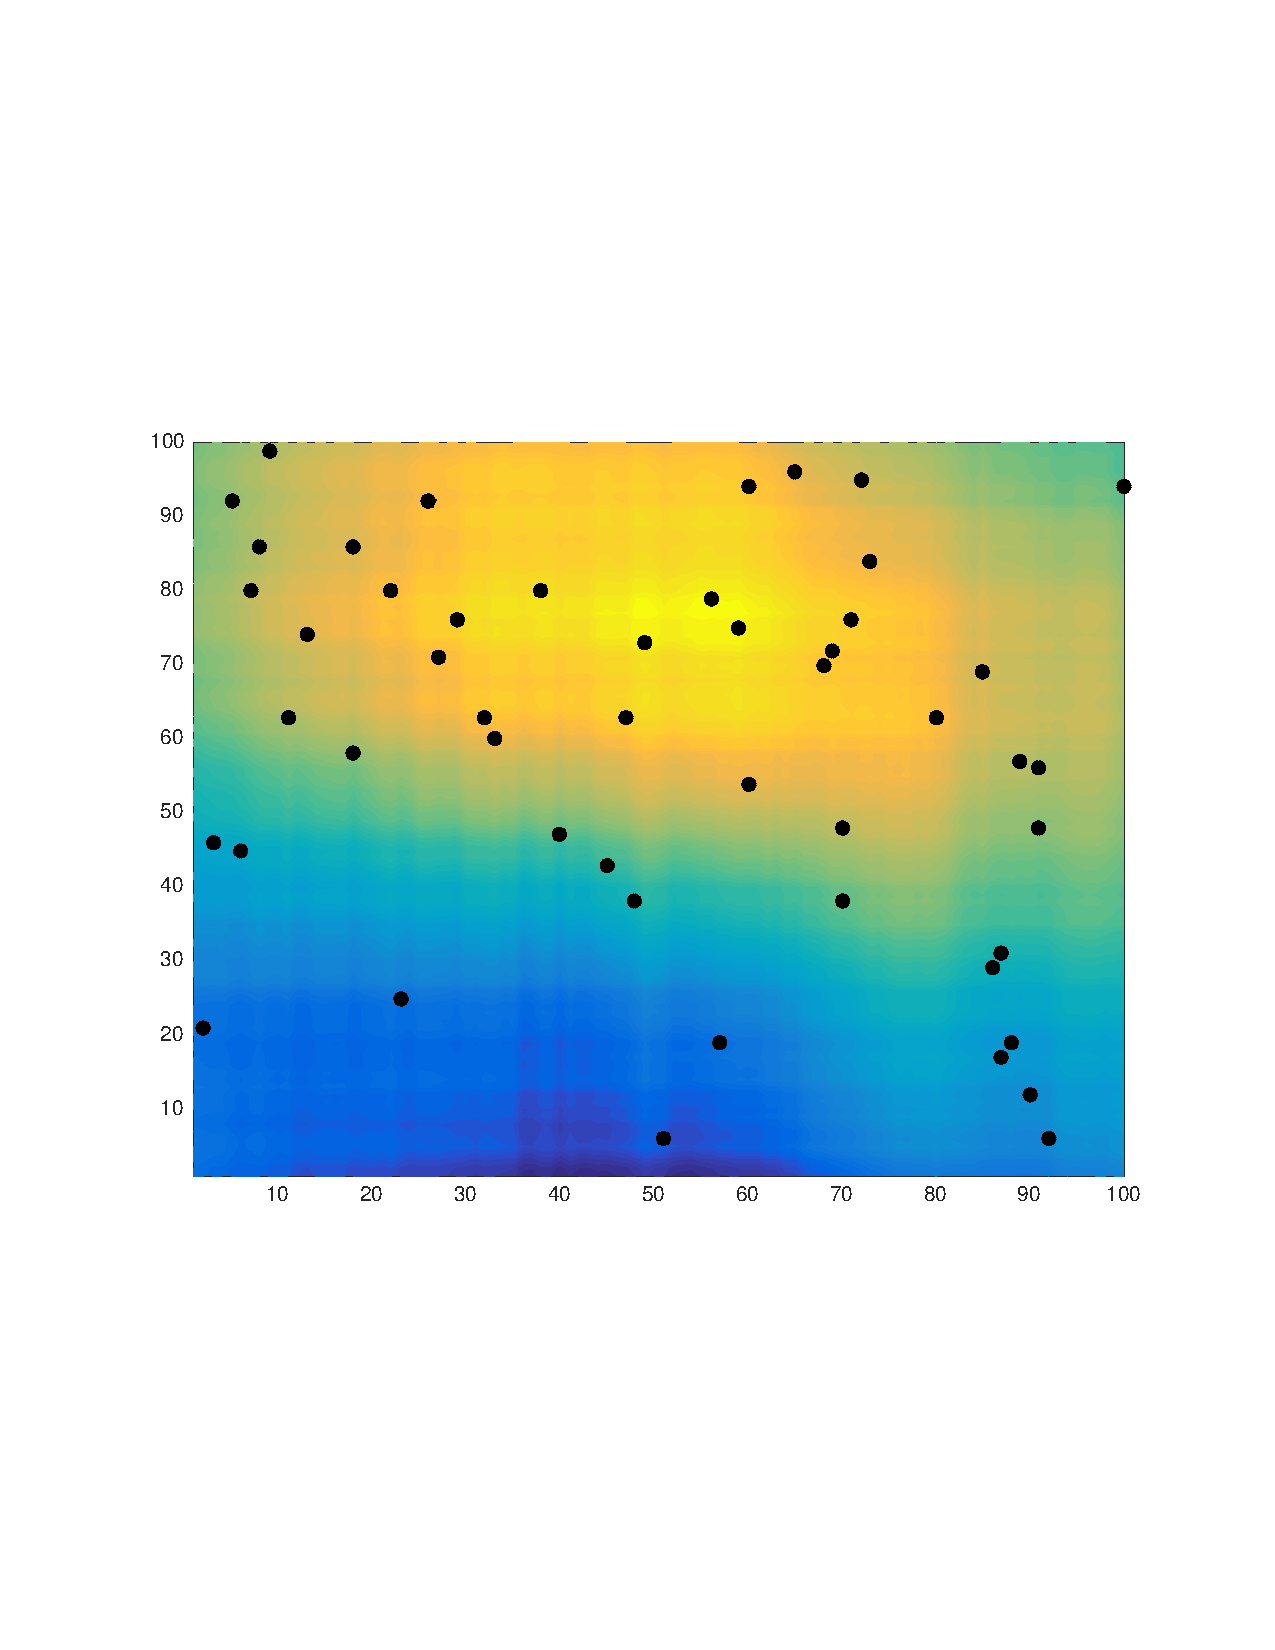
\includegraphics[width=\linewidth]{figures/sampled_generated_field.png}
        \captionsetup{skip=0.5\baselineskip, width=0.8\textwidth, size=footnotesize}
        \caption{Sampled locations (250 points marked in black) of the previously generated geospatially autocorrelated field in Figure \ref{fig:top_view_field}}
        \label{fig:samples}
    \end{subfigure}%
    ~ 
    \begin{subfigure}[t]{0.5\textwidth}
        \centering
        \includegraphics[width=\linewidth]{figures/idw_predicted_field.png}
		\captionsetup{skip=0.5\baselineskip, width=0.8\textwidth, size=footnotesize}
		\caption{An Inverse Distance Weighting generated predicted field ($p=3$). Generated from 250 random observations made in Figure \ref{fig:samples}}
		\label{fig:idw_field}
    \end{subfigure}
    \\
    \begin{subfigure}[t]{0.5\textwidth}
        \centering
        \includegraphics[width=\linewidth]{figures/generated_field_side_view.png}
        \captionsetup{skip=0.5\baselineskip, width=0.8\textwidth, size=footnotesize}
        \caption{A side view of the previously generated geospatially autocorrelated field in Figure \ref{fig:side_view_field}}
    \end{subfigure}%
    ~
    \begin{subfigure}[t]{0.5\textwidth}
        \centering
        \includegraphics[width=\linewidth]{figures/idw_side_pred_field.png}
        \captionsetup{skip=0.5\baselineskip, width=0.8\textwidth, size=footnotesize}
        \caption{A side view of the IDW generated in Figure \ref{fig:idw_field}}
    \end{subfigure}
    \captionsetup{skip=0.5\baselineskip,size=footnotesize}
    \caption{A randomly generated field where 250 observations were made (left), and an Inverted Distance Weighted Prediction (right) of that field}
    \label{fig:idw_side_by_side}
\end{figure*}

This method can give us a prediction for all possible $\vect{X}_j$ points in a field where a set of observations at labeled positions were made, as done in Figure \ref{fig:idw_side_by_side}. Unfortunately, the method is limited in that it does not take advantage of the underlying stochastic model of the field, $Z$, being observed. We will further expand on this method to exploit the fact that $Z$ is a stochastic process with underlying geospatially autocorrelated random variables.

\section{Variography}
Variography is a set of procedures for examining and interpreting spatial dependence and geospatial autocorrelation in observed data. We would like to unravel the autocorrelation, or spatial dependence, of observed data to factor into a classical Inverse Distance Weighting, yielding a Best Linear Unbiased Predictor. The heart of variography is the Variogram Function, a function which quantifies dependence for observed data separated by some vector distance and angle, i.e. the covariance between two given points in a stochastic field. We will develop the basis for the Variogram function and fit our sampled observations to a continuous Variogram model.

\subsection{The Variogram}
A Variogram is intended to be a continuous function which yields a covariance between two points $Z(\vect{X}_{i})$, $Z(\vect{X}_{j})$, which were not nessecarilly observed, but known to be a vector $\vect{h} \in \mathbb{R}^2$ apart. Using the assumption made in Equation 2.4.1 of Matherson, 1963 \cite{matheron:geostat}:

\begin{equation}
    Z(\vect{X}_i)=\mu(\vect{X}_i)+\delta(\vect{X}_i)
    \label{eq:matheron:assum}
\end{equation}

Where $\delta(\cdot)$ is a zero-mean intrinsically stationary stochastic process, which our observations in a field $Z$ are therefore expected to be. If we assume a mean $\mu(\cdot)$ is only constant in a reasonably small neighborhood, a modified version of the variogram definition in equation 2.3.4 of Matherson, 1963 \cite{matheron:geostat} is defined to be:

\begin{equation}
	2\gamma(\vect{X}_i, \vect{X}_j)= \text{var} (Z(\vect{X}_{i}) - Z(\vect{X}_{j}))=E[( (Z(\vect{X}_{i}) - \bar{Z} ) - (Z(\vect{X}_{j}) - \bar{Z} ))^2]
    \label{eq:cont_var}
\end{equation}

Where $\bar{Z}$ is the mean of the observations made in a stochastic field, $Z$, for a reasonably small neighborhood of points.

It is infeasible and impossible to estimate an observation value at each possible point to compute a continuous variogram. We must therefore define a discrete model which will be fit into a continuous variogram model.

\subsection{The Semi-Variogram}
A Semi-Variogram, or Experimental Variogram, is a discrete function representing the covariance of the observation value difference between two sampled locations that are some vector $\vect{h}$ apart. By modifying equation 2.4.2, Matheron, 1963 \cite{matheron:geostat} to include an additional boundery to classify a "bin", for two observations $\vect{X}_{i}$, $\vect{X}_{j}$ in a stochastic field, $Z$, the experimental semivariogram is defined to be:

\begin{equation} 
    \label{eq:exp_var}
    2\hat{\gamma}(\vect{h}+\vect{\delta}) := \frac{1}{|N(\vect{h}+\vect{\delta})|}\sum\limits_{(i,j)\in N(\vect{h}+\vect{\delta})}|Z(\vect{X}_i) - Z(\vect{X}_j)|^2 % (Cressie 1993)
\end{equation}

Where $N(\vect{h}+\vect{\delta})$ are the pairs of observed data locations that are a vector distance and angle, commonly referred to as a \textit{lag}, $\vect{h}+\vect{\delta}$ apart, $|\cdot|$ is the finite cardinality of such a set, and $\vect{\delta} = \begin{bmatrix}\pm\delta & \pm\delta\end{bmatrix}^{T}$ is a bound of ranges acceptable to be "binned" alongside $\vect{h}$.

\begin{figure}[H]
    \centering    
    \includegraphics[width=\linewidth]{figures/exp_variogram.png}
    \captionsetup{skip=0.5\baselineskip,size=footnotesize}
    \caption{An experimental variogram generated using Equation \ref{eq:exp_var} on the field and random samples previosuly generated in Figure \ref{fig:samples}. $\delta$ was chosen such that for $n$ observations, a total number of $\Big\lfloor \frac{n}{2} \Big\rfloor$ points were plotted}
    \label{fig:exp_var}
\end{figure}

The plot of the experimental variogram in figure \ref{fig:exp_var} conveys to us the geospatial autocorrelation of the sampled field that was previously generated in figure \ref{fig:samples}. We can see that as the distance, $\|\vect{h}\|_2$, between two given points increases, the covariance also increases. At some point in the graph the covariance levels out to a steady value (the sill) at some distance in the domain (the range). This informs us of locations of where the loss of reliable geospatial autocorrelation between two points that are a vector distance $\vect{h}$ apart lies. This will later act as a method of prediction confidence in our Best Linear Unbiased Predictor.

\subsection{Converting a Semi-Variogram to a Variogram}
The intent of fitting a statistical model to an experimental variogram is to approximate the continuous covariance for any two points on $Z$ that are at some known $\vect{h}$ apart. This will allow us to obtain a decent approximation of the continuous Variogram function in equation \ref{eq:cont_var}. In order to define the experimental semi-variogram to variogram procedure, we must first define the \textit{range}, \textit{sill}, and \textit{nugget} characteristics of a variogram. The value on the co-domain where the variogram begins to flatten out (approximately a zero derivative variance) is referred to as the sill. The sill variance value associated with the sill is the largest variability between any two data pairs in the field. The cooresponding point on the distance domain is called the range. It is important to note that a lag larger than the range is not spatially autocorrelated \cite{felus:srn}. The nugget is defined to be the variance at zero separation. This value is exactly zero for ideal measurments, but is generally not for real-life measurments.

\subsection{Variogram Models}
Our variogram can take on the form of one of multiple well known "kernels", or statisticals models. All of which are scalar functions of the range, $a$, and sill, $s$, of our lag distribution model, and scalar $h = \|\vect{h}\|_2$. The three most common models are the following: %P. Goovaerts. Geostatistics for natural resources evaluation. Oxford University Press, New York, 1997.
\subsubsection{The Gaussian Model}

\begin{equation}
	\gamma(h, s, a) = s \Bigg[ 1 - \exp \Bigg( -\dfrac{h^2}{a^2} \Bigg) \Bigg]
	\label{eq:gauss_model}
\end{equation}

The Gaussian models will asymptotically reach its sill. The \textit{practical range} is then used to refer the point on the domain where the variogram reaches 95\% of its sill.

\subsubsection{The Exponential Model}

\begin{equation}
	\gamma(h, s, a) = s \Bigg[ 1 - \exp \Bigg( \dfrac{h}{a} \Bigg) \Bigg]
	\label{eq:exp_model}
\end{equation}

The same rules as the Gaussian model apply to the Exponential model.

\subsubsection{The Spherical Model}

\begin{equation}
	\gamma(h, s, a) = \frac{s}{2} \Bigg[ \dfrac{3h}{a} - \Bigg( \dfrac{h}{a} \Bigg)^3 \Bigg]
	\label{eq:sph_model}
\end{equation}

The spherical model will reach an exactly zero slope at the sill and range.

\subsection{Fitting A Semi-Variogram}

Though there exists no closed-form solution for obtaining a continuous variogram, we will use a nonlinear programming solver which searches for the minimum error in:

\begin{equation}
\min\limits_{h, s, a}\gamma(h, s, a)
\end{equation}

We specifically will use a modified (we specified bounds to decrease iterations of the function fit) \textit{fminsearch} function in \textit{MATLAB} which is defined to "find the minimum of unconstrained multivariable function using a derivative-free method". This is done by specifying an objective function to minimize (our desired statistical model) over our experimental semi-variogram.

\begin{figure}[ht!]
    \centering    
	\includegraphics[width=\linewidth]{figures/fit_kern_comp.png}
	\captionsetup{skip=0.5\baselineskip,size=footnotesize}
	\caption{A comparison of the Gaussian, Spherical, and Exponential statistical models fit to the Experimental Semi-Variogram in Figure \ref{fig:exp_var}}
	\label{fig:kern_fit}
\end{figure}

\subsection{Variance-Covariance Matrix}
From the fit variogram which represents our lag variances, we will construct a \textit{variance-covariance matrix}, $C_n$. The matrix will contain all of the relevant relationships required to interpolate a given neighborhood of a field from $n$ observations. The value of the element $C_{i,j}$, will represent the variance of the lag between the $i^{th}$ and $j^{th}$ observations, measured from the fit variogram.

\subsection{The Proximity Vector}
For any given point on a field, we can construct a \textit{proximity vector}, $d_n \in \mathbb{R}^n$, which contains the variance of a given point on the field with all of the $n$ observations made. The $k^{th}$ element of $d_n$, for a point ($i,j$) on the field, contains the variance for the lag between coordinate $\begin{bmatrix} i & j \end{bmatrix}^{T}$ on the field and the $k^{th}$ observation made, where $1 \leq k \leq n$.

\section{The Kriging Method}
\subsection{A Best Linear Unbiased Predictor}
\subsection{Exploiting Geospatial Autocorrelation}
\section{Forms of the Kriging Method}
\section{The Kriging Formula}
\section{The Kriging Prediction}

\begin{figure*}[ht!]
    \centering
    \begin{subfigure}[t]{0.5\textwidth}
        \centering
        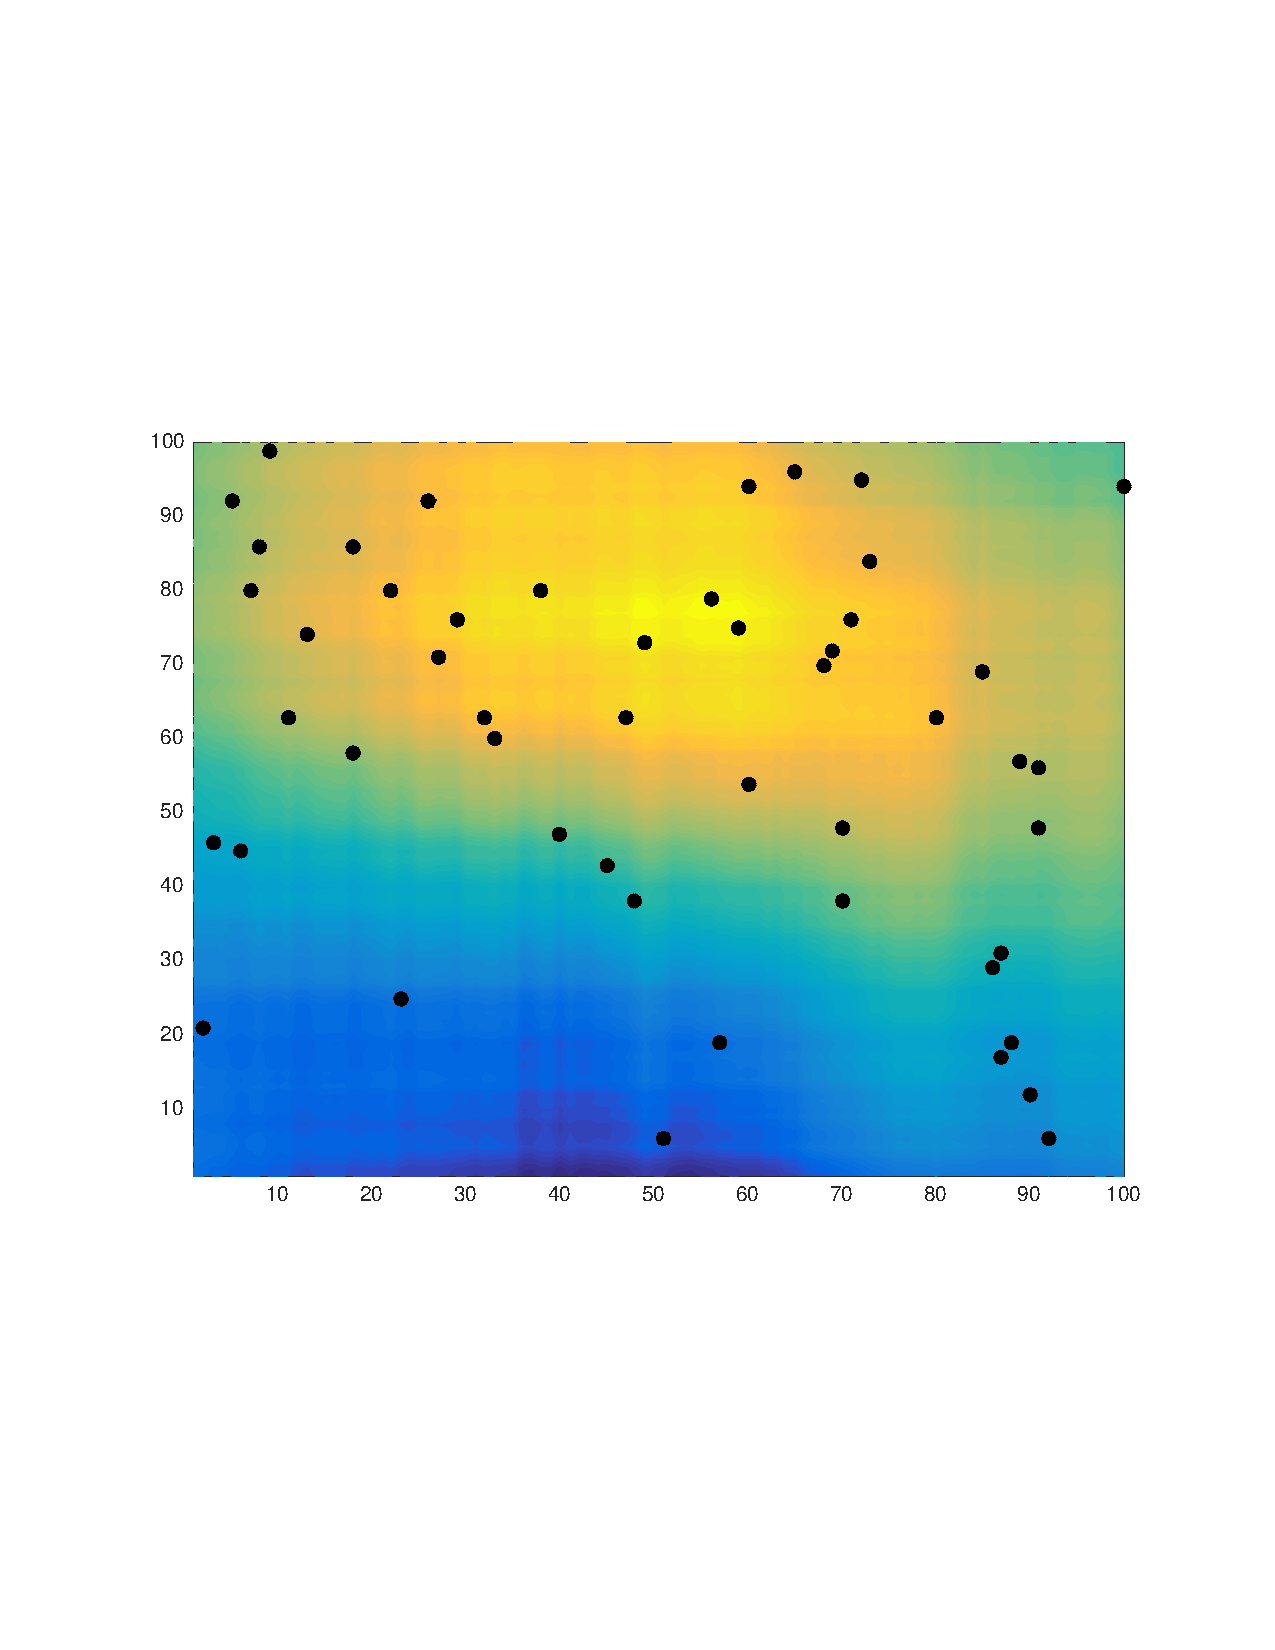
\includegraphics[width=\linewidth]{figures/sampled_generated_field.png}
        \captionsetup{skip=0.5\baselineskip, width=0.8\textwidth, size=footnotesize}
        \caption{Sampled locations (250 points marked in black) of the previously generated geospatially autocorrelated field}
        \label{fig:sampled_field}
    \end{subfigure}%
    ~ 
    \begin{subfigure}[t]{0.5\textwidth}
        \centering
        \includegraphics[width=\linewidth]{figures/kriging_top_pred_field.png}
        \captionsetup{skip=0.5\baselineskip, width=0.8\textwidth, size=footnotesize}
        \caption{A Kriging Prediction of the originally generated random field}
        \label{fig:krig_field}
    \end{subfigure}
    \captionsetup{skip=0.5\baselineskip,size=footnotesize}
    \caption{A randomly generated field where 250 observations were made (left), and a Kriging Prediction (right) of that field from the marked observations.}
    \label{fig:krig_side_by_side}
\end{figure*}

\begin{figure*}[ht!]
    \centering
    \begin{subfigure}[t]{0.5\textwidth}
        \centering
        \includegraphics[width=\linewidth]{figures/generated_field_side_view.png}
        \captionsetup{skip=0.5\baselineskip, width=0.8\textwidth, size=footnotesize}
        \caption{A side view of the previously generated geospatially autocorrelated field}
        \label{fig:sampled_field}
    \end{subfigure}%
    ~ 
    \begin{subfigure}[t]{0.5\textwidth}
        \centering
        \includegraphics[width=\linewidth]{figures/kriging_side_pred_field.png}
        \captionsetup{skip=0.5\baselineskip, width=0.8\textwidth, size=footnotesize}
        \caption{A Kriging Prediction of the originally generated random field}
        \label{fig:krig_side_field}
    \end{subfigure}
    \captionsetup{skip=0.5\baselineskip,size=footnotesize}
    \caption{A randomly generated field where 250 observations were made (left), and a Kriging Prediction (right) of that field from the marked observations.}
    \label{fig:krig_side_side_by_side}
\end{figure*}

\subsection{Kriging Variance}
%Interpolation Accuracy

\chapter{Optimization of Interpolation Methods}
Although the method is optimal for data with no trends or drift, the use of the unmodified Kriging Method technique has the drawback of being computationally intensive and slow to compute in a live and timely manner. This is due to the multiple matrix inversions and least squares fittings required to calculate the weights of the interpolation from the continuous variograms. It would be desired, in the case of autonomous UAVs that must constantly steer themselves in the best direction, to quickly calculate probabilities and variances. We will further discuss methods of efficient interpolation using the Universal Kriging Method.
\section{Natural Neighbor Selection}
\subsection{Voronoi Tessellations}
\subsection{Finding Natural Neighbors}

\chapter{Required Graph Theory}
\section{Graph Construction}
\subsection{Vertices and Edges}
\subsection{Path Problems}
\subsubsection{Optimizing a Route}

\chapter{Previous Work}
Some other research was once performed.

\chapter{Live Aerial Interpolation}

\chapter{Live Autonomous Path Finding}
We know for a geospatially autocorrelated field there is a stochastic process underlying in the data we would like to predict, and therefore could interpolate further based off of the variances of two disjoint points in the field. The variances, from samples collected in the scanning process which factor into our variogram, then become our relative confidence scores of predictions in our field in question. The values in the variogram are what will be used to terminate the interpolation when a level of least-confidence in total prediction is achieved, and what will dictate the future scan locations for a UAV or a pod of UAVs.
\subsection{Constructing a Confidence Graph}
\subsection{Confidence Optimized Path Finding}

\part{Simulation}
\subsection{Flying Engine}
\subsubsection{Plot Drawing}
\subsubsection{Way-point Selection}

\section{FastPAS}
\subsection{The Algorithm}
\subsection{Simulating It}

\section{Other Uses}
% real estate
% crypto price pred.
% gentrify

\chapter{Results}

\chapter{Conclusion}
The method has proven to be a powerful interpolation method in simulations for simulated fields. The Kriging method has proven to be a working aerial mapping technique that provides a robust model for predictions and confidence scores. The goal of this thesis will be to design the algorithm for use with a pod of autonomous UAVs. A modified technique will have to first be developed to reduce the computational complexity of the algorithm by autonomously selecting optimal neighborhoods of sub-areas to run the method on.\\
Once the new method has been developed, an accurate simulation demonstrating its effectiveness and potential to be used in a real pod of UAVs will then be created and demonstrated. 
If time and resources are available, the algorithm will be ported to a real pod of UAVs to accomplish the task of autonomous scanning using thermal imaging (via infrared sensors). Tests will be conducted to prove the effectiveness and time efficiency of the newly developed algorithm.

\nocite{*}
\bibliographystyle{plain}
\bibliography{yonan_cmpe_msc_thesis}

\appendix
\chapter{Ancillary Material}

\end{document}
